\documentclass[a4paper,12pt,titlepage,margin=1in]{article}
\usepackage{graphicx}
\usepackage[hidelinks]{hyperref}
\usepackage{listings}
\usepackage{float}
\DeclareGraphicsExtensions{.png, .jpg}

\begin{document}
%\title and intnro
\begin{titlepage}
	\begin{center}
		
		\begin{figure}[t]
			\centering
			
\includegraphics[width=450px]{./Graphics/KPTH_Logo}
		\end{figure}		
		
		\textbf{\LARGE Gynaecological Patient Information
		Management System:}
		
		\vspace{1 cm}
	    \textbf{\LARGE \\Software Test Documentation}
		
		\vspace{1 cm}
		\LARGE{\textbf{Team Pentec: }}
		

		\begin{flushright} \large
			
			Ruth Ojo 12042804\newline
			Liz Joseph 10075268\newline
			Trevor Austin 11310856\newline
			Maria Qumayo 29461775\newline
			Lindelo Mapumulo 12002862\newline
		\end{flushright}
		
				\vspace{1 cm}
				\centering
				
\includegraphics[width=150px]{./Graphics/Pentec_Logo.png}

		
		
		{\LARGE Final Version}
		\\
		{\large \today}		
		
		
	\end{center}
\end{titlepage}

%\table of content
\tableofcontents
\newpage

\section{INTRODUCTION}  
%\Intro
	\subsection{Objectives}
		The following doucment contains the detailed outline of the PIMS testing process and results. Bellow are the main modules that were tested.
\begin{itemize}
	\item User Login
	\item PIMS Artificial Intelligence
	\item PIMS Statistics
	\item PIMS Notifications
	\item PIMS Space
\end{itemize}

Testing was done on the system mainly for the following 5 reasons:

\begin{itemize}
	\item To ensure that the system meets both functional and non functional requirements arroding to the given spesifications
	\item System stress, that is to make sure that the system does not fail with multiple users or any other factors because it is expensive to resolve and fix at a later stage.
	\item To handle and resolve System failures and bugs appropriatly and in good time.
	\item To point out the defects and errors that were made during and after the development phases.
	\item To ensure that the final product is of top, professiona, software engineering standards.
\end{itemize}

	\subsection{Testing Strategy}
		\subsubsection*{Our approach}
Different strategies were conducted for the different kinds of testing. 
All strategies were decided upon according to according to the level of the test	
\subsubsection*{Mechanism}	
\begin{enumerate}
\item Strategy:
	\begin{itemize}
		\item Open-source resources: using open source resources to minimize our individual costs.
		\item Iterative development and regular reviews: This will help us improve system quality so we were able to change and update any errors upon first encounter.
	\item Documentation and tracking: The relevant documentation to keep track of our findings.
\end{itemize}

%	\subsection{Scope}	
%	\subsection{Reference Material}
%	\subsection{Definitions and Acronyms}
	

%\section{TEST ITEMS}
%	\subsection{Program Modules}
%	\subsection{Job Control Procedures}
%	\subsection{User Procedures}
%	\subsection{Operator Procedures}
	
\section{FEATURES TO BE TESTED (Functional Requirements)}
	\subsection{PIMS Login}
	%By Maria/
 \subsubsection{Pims Login}
Pims User login testes for correct authentication and identification before the user is allowed system access. Further testing was done for user rights and privilages.
\newline

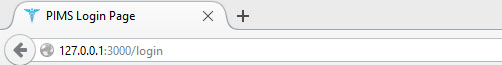
\includegraphics[width=\linewidth]{./Graphics/login.jpg}
\newline

Front end representation
\newline

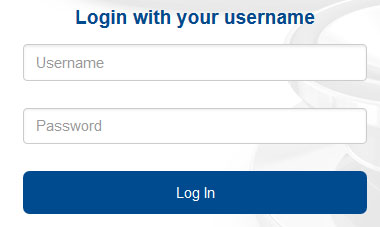
\includegraphics[width=\linewidth]{./Graphics/frontEnd.jpg}
		
User Authentication tested for the following conditions					
	\begin{itemize}
				\item Provide user with access
				\item Retrieve username
				\item Retrieve user password
				\item Fail with empty username and/ or empty password
				\item Return a boolean with regards to user right.
 \end{itemize}
 
 The figure bellow depics the successful testing of the Authentication and checkAdmin functions.
 \newline
 
 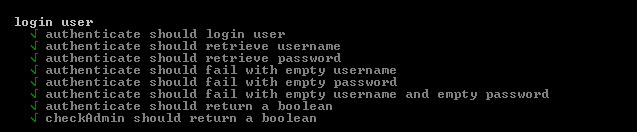
\includegraphics[width=\linewidth]{./Graphics/userResults.jpg}
 
 \subsubsection{Remarks}
 	\begin{itemize}
 				\item Pre-Conditions
 		User does not have access to systme.
 				\item Post-Conditions
 With correct login details, user successfuly gains access into the system with.
 User rights are checked upon login authentication
  \end{itemize}
  
  Both Pre and Post conditions  are considered in the implimentation of the system login. Unit testing successfuly.  tested with no violations to the security of the systm.
 
	\subsection{PIMS Notifications}
	%By Maria/
 \subsubsection{Pims Login}
Pims Send Notification is a two part function that we tested. First check if user is found(exists) in the database. Then send email using smtp.The unit test codes bellow demonstrates.
\newline

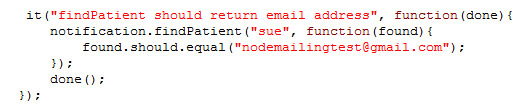
\includegraphics[width=\linewidth]{./Graphics/find.jpg}
\newline

Send Notifications via email
\newline

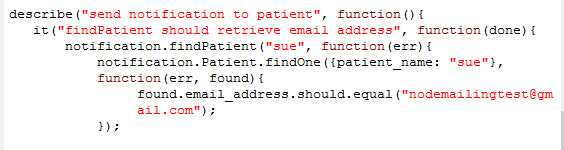
\includegraphics[width=\linewidth]{./Graphics/send.jpg}
The following conditions must be true for the send notification use case to pass.					
	\begin{itemize}
				\item Find patient should query the database to see if a user exists by searching for an email adress.
				\item Oce user is found, send notification must send and email to the found adress.
 \end{itemize}
 
 The figure bellow depics the successful testing of the Send Notification and FindUser functions.
 \newline
 
 \includegraphics[width=\linewidth]{./Graphics/Notify.jpg}
 
 \subsubsection{Remarks}
 	\begin{itemize}
 				\item Pre-Conditions
 		User must exist in database and have and email.
 				\item Post-Conditions
	User recieves and email from Prof Snyman.
  \end{itemize}
  
  Both Pre and Post conditions  are considered in the implimentation of sending notifications. Unit testing successfuly.  tested with no violations to the security of the systm.
 
	\subsection{PIMS Edit Profile}
	%By Maria/
 \subsubsection{Pims Login}
Pims edit user profile should be able to allow the admin user to update his profile and edit his information accordingly.
\newline

The Code bellow demonstrates the update of the user name after retrienving it.
\newline
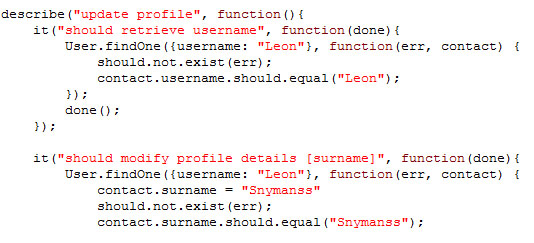
\includegraphics[width=\linewidth]{./Graphics/editCode.jpg}
\newline
		
Edit profile was  tested for the following conditions					
	\begin{itemize}
				\item Retrieve data
				\item Modify profile details
 \end{itemize}
 

 The figure bellow depics the successful testing of the UpdateAuthentication and checkAdmin functions.
 \newline
 
 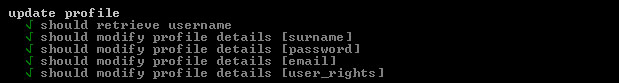
\includegraphics[width=\linewidth]{./Graphics/editProfile.jpg}

 
	\subsection{PIMS Add User}
	
Adding a user, is a feature only available for the admin user and is a crucial use-case needed for saving a new user’s to the system.
\newline
\newline
The add user case passed unit testing successfully as seen in the figure bellow
\newline
\newline
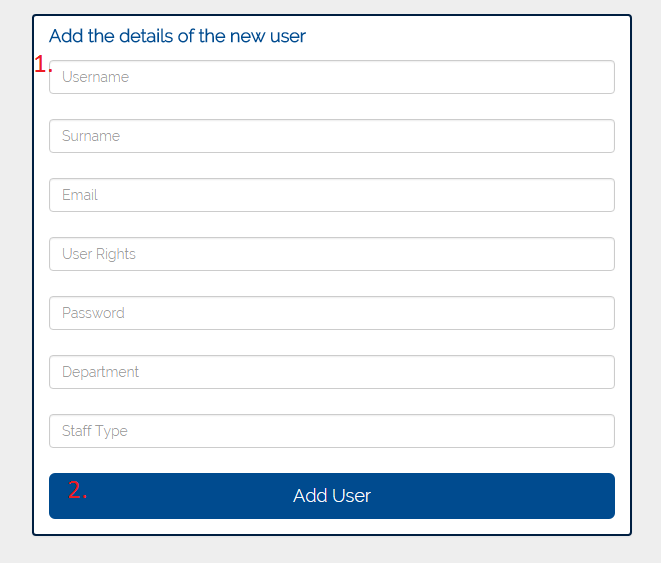
\includegraphics[width=350px]{./TestingDoc/Graphics/addUser}
\newline		
\subsubsection*{Conditions}
The following pre and post conditions are defined for adding a new user.
\newline
\newline	
\subsubsection*{Pre conditions}	
\begin{itemize}
		\item User must be logged in as admin.
		\item User to be added must not already exist in the database.
		\item User must be a medical personnel.
\end{itemize}	

\subsubsection*{Post conditions}	
\begin{itemize}
		\item New user is added and can interact with the system.
\end{itemize}	

The code bellow shows the testing for adding a new user with sample data	
\newline
\newline
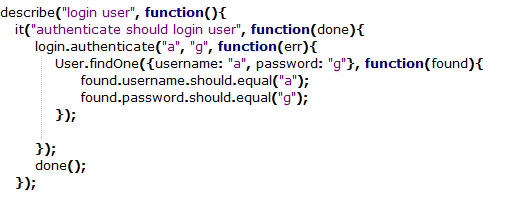
\includegraphics[width=350px]{./TestingDoc/Graphics/UserMustLogIn}

\subsubsection*{Remark}
Add User unit test successfully passes.
	\subsection{PIMS Statistics}
	%By Maria
\subsection{Login and Admnistartive user}
	\subsubsection*{PIMS Login}
		Functional Testing
		- for each use case tested
		* either success or a list of violations of the contract requirements (pre- and post-condition violations or data structure requirements)
		* a test coverage analysis reporting which percentage of the use cases have been covered by the testing
		
		2. Non-functional testing/assessment
		- any performance, scalability, maintainability, reliability, usability, ... problems identified with evidence for the identified problem.
	
				
					\begin{itemize}
							\item The Buzz Space system has to accommodate and host a multitude of users concurrently, thus making it prone to various malfunctions and glitches
							
							\item The Space needs to be monitored in real time at all times to ensure relevance of topics and subject matters.
							\item The rating and tagging functionality need to be fair and accurate
							
							\item Sufficient feedback and updates of the Buzz Space state must be provided to the users. Users that create threads or just comment on one.
							
							\item General software control and application usage..
						 \end{itemize}
	
%\section{FEATURES NOT TO BE TESTED (Non-Functional Requirements)}
	%\subsection{Usability}
%	\subsection{Scalability}
%	\subsection{Performance}
%	\subsection{maintainability}
%	\subsection{Reliability}
%	\subsection{Secutity}
%	\subsection{Monitorability}
%	\subsection{Extendability} 

%\section{APPROACH}
%	\subsection{Component Testing}
%	\subsection{Integration Testing}
%	\subsection{Conversion Testing}
%	\subsection{Job Stream Testing}
%	\subsection{Interface Testing}

%	\subsection{Recovery Testing}
%	\subsection{Performance Testing}
%	\subsection{Regression Testing}
%	\subsection{Acceptance Testing}
	
%\section{PASS / FAIL CRITERIA}
%	\subsection{Suspension Criteria}
%	\subsection{Resumption Criteria}
%	\subsection{Approval Criteria}
		
%\section{Testing Process}
%	\subsection{Test Deliverables}
%	\subsection{Testing Tasks}
%	\subsection{Responsibilities}
%	\subsection{Resources}
%	\subsection{Schedule}
	
%\section{Environmental Requirements}
%	\subsection{Hardware}
%	\subsection{Software}
%	\subsection{Security}
%	\subsection{Tools}
%	\subsection{Publications}
%	\subsection{Risks and Assumptions}

%\section{Change Management Procedures}

%\section{Remarks}
%	\subsection{Risks and issues}
%	\subsection{Product quality}
%	\subsection{Possible improvements}

%\section{Conclusion}
	

\end{document}